\section*{Zadanie 40.}
\begin{task}
Fala płaska rozchodząca się w kierunku $+Ox$ pada prostopadle na granice w układzie trzech ośrodków:\\
I $\hspace{1cm}$ $\varepsilon_{1}=\epsilon_{0} \hspace{1.2cm} \mu_{1}=\mu_{0} \hspace{1cm} \sigma=0 \hspace{4cm}$ dla $x<-d$\\
II $\hspace{0.86cm}$ $\epsilon_{2}=3\epsilon_{0} \hspace{0.95cm} \mu_{2}=? \hspace{1.35cm} \sigma=0 \hspace{4cm}$ dla $-d\le x<0$\\
III $\hspace{0.72cm}$ $\epsilon_{3}=? \hspace{1.4cm} \mu_{3}=5\mu_{0} \hspace{0.83cm} \sigma=0 \hspace{4cm}$ dla $0\le x$\\
gdzie d=7.5cm.\\
Wiedząc, że współczynnik fali stojącej w ośrodku I wynosi jeden w zakresie częstotliwości od 8 GHz do 12 GHz wyznaczyć wartości $\mu_{2}$ i $\epsilon_{3}$. Dla częstotliwości 10GHz obliczyć długość fali w ośrodku II i narysować obwiednię natężenia pola elektrycznego znormalizowaną do amplitudy $E_{30}$ natężenie pola elektrycznego fali w ośrodku III.\\
\end{task}

\begin{solution}

\textbf{Obliczanie parametrów ośrodka:}
$$WFS_{1}=1 \ \ \ \implies \ \ \ \Gamma_{1,2}=0$$
$$\Gamma_{1,2}=0 \ \ \ \implies \ \ \ Z_{in}=Z_{1} \ \ \ \implies \ \ \ Z_{2}\cfrac{Z_{3}+jZ_{2}\tg{\beta_{2}d}}{Z_{2}+jZ_{3}\tg{\beta_{2}d}}=Z_{1}$$
$\left\{ \begin{array}{l} Z_{1}=\sqrt{\cfrac{\mu_{1}}{\epsilon_{1}}}Z_{0}\\Z_{2}=\sqrt{\cfrac{\mu_{2}}{\epsilon_{2}}}Z_{0}\\Z_{3}=\sqrt{\cfrac{\mu_{3}}{\epsilon_{3}}}Z_{0}  \end{array} \leftarrow \ \mu_{x} \ \epsilon_{x}$ traktujemy jako liczby, współczynniki przy $\epsilon_{0} \ \mu_{0}$ \\ Podstawiamy i wymnażamy obie strony przez mianownik:\\
$$\sqrt{\cfrac{\mu_{2}}{\epsilon_{2}}}Z_{0}\big{(}\sqrt{\cfrac{\mu_{3}}{\epsilon_{3}}}Z_{0}+j\sqrt{\cfrac{\mu_{2}}{\epsilon_{2}}}Z_{0}\tg{\beta_{2}d}\big{)}=\sqrt{\cfrac{\mu_{1}}{\epsilon_{1}}}Z_{0}\big{(}\sqrt{\cfrac{\mu_{2}}{\epsilon_{2}}}Z_{0}+j\sqrt{\cfrac{\mu_{3}}{\epsilon_{3}}}Z_{0}\tg{\beta_{2}d}\big{)}$$
$$\sqrt{\cfrac{\mu_{2}\mu_{3}}{\epsilon_{2}\epsilon_{3}}} +j\cfrac{\mu_{2}}{\epsilon_{2}}\tg{\beta_{2}d} = \sqrt{\cfrac{\mu_{1}\mu_{2}}{\epsilon_{1}\epsilon_{2}}}+j\sqrt{\cfrac{\mu_{1}\mu_{3}}{\epsilon_{1}\epsilon_{3}}}\tg{\beta_{2}d} $$
Porównujemy liczby zespolone ($ \Re(z_{1})=\Re(z_{2}) $ oraz $ \Im(z_{1})=\Im(z_{2})$) i podstawiamy wartości liczbowe! ($\epsilon_{0}$ oraz $\mu_{0}$ skróciliśmy w $Z_{0}$)\\
$$\left\{ \begin{array}{l} \sqrt{\cfrac{5\mu_{2}}{3\epsilon_{3}}}=\sqrt{\cfrac{\mu_{2}}{3}}\\ \cfrac{\mu_{2}}{3}=\sqrt{\cfrac{5}{\epsilon_{3}}} \end{array}\ \ \ \implies \ \ \  \left\{ \begin{array}{l} \epsilon_{3}=5\\ \mu_{2}=3 \end{array}$$\\
\textbf{Obliczanie długości fali w ośrodku 2:}
$$ \cfrac{\omega}{\beta} = \cfrac{1}{\sqrt{\mu\epsilon}}\ \ \ \implies \ \ \ \beta=\cfrac{\omega}{\cfrac{1}{\sqrt{\mu\epsilon}}}, \ \ \ \ \lambda=\cfrac{2\pi}{\beta} $$
$$ \beta_{2}=\cfrac{3\omega_{2}}{c}=200\pi\ \ \ \ \implies \lambda_{2}=\cfrac{2\pi}{200\pi}=0.01m $$
	\begin{center}
    $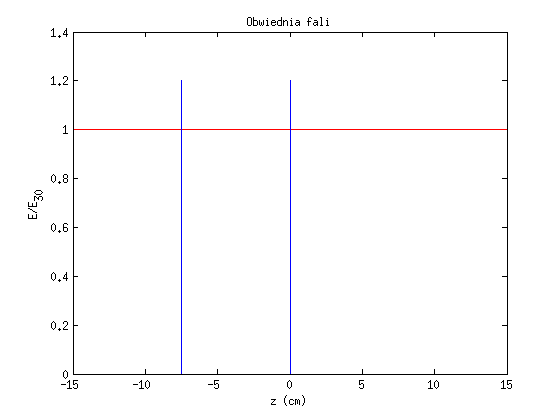
\includegraphics[scale=1]{40}$\\
    \end{center}

\end{solution}